\iffalse
\documentclass[12pt]{article}
\usepackage{graphicx}
\usepackage[none]{hyphenat}
\usepackage{graphicx}
\usepackage{listings}
\usepackage[english]{babel}
\usepackage{graphicx}
\usepackage{caption} 
\usepackage{booktabs}
\usepackage{array}
\usepackage{amssymb} % for \because
\usepackage{amsmath}   % for having text in math mode
\usepackage{extarrows} % for Row operations arrows
\usepackage{listings}
\lstset{
  frame=single,
  breaklines=true
}
\usepackage{hyperref}
  
%Following 2 lines were added to remove the blank page at the beginning
\usepackage{atbegshi}% http://ctan.org/pkg/atbegshi
\AtBeginDocument{\AtBeginShipoutNext{\AtBeginShipoutDiscard}}


%New macro definitions
\newcommand{\mydet}[1]{\ensuremath{\begin{vmatrix}#1\end{vmatrix}}}
\providecommand{\brak}[1]{\ensuremath{\left(#1\right)}}
\providecommand{\norm}[1]{\left\lVert#1\right\rVert}
\providecommand{\abs}[1]{\left\vert#1\right\vert}
\newcommand{\solution}{\noindent \textbf{Solution: }}
\newcommand{\myvec}[1]{\ensuremath{\begin{pmatrix}#1\end{pmatrix}}}
\let\vec\mathbf


\begin{document}

\begin{center}
\title{\textbf{Conic Sections - Ellipse}}
\date{\vspace{-5ex}} %Not to print date automatically
\maketitle
\end{center}
\setcounter{page}{1}

\section{11$^{th}$ Maths - Chapter 11}
This is Problem-7 from Exercise 11.5
\begin{enumerate}

\solution 
\fi
The conic section for the given problem is an ellipse. Let $\vec{O}\myvec{0 \\ 0}$ be the centre of the Ellipse. Then, the focii are given by 
\begin{align}
    \label{eq:chapters/11/11/5/7/ellipseEq1}
	\vec{F_1} = \myvec{ 4 \\ 0} \\
	\vec{F_2} = \myvec{ -4 \\ 0} 
\end{align}
The sum of the distances from two focii to the point on the locus of the ellipse is equal to $10m$. Let $\vec{P}\myvec{p \\ 0 }$ and $\vec{Q}\myvec{-q \\ 0}$ be the vertices of the ellipse. Then
\begin{align}
	\norm{\vec{P}-\vec{F_1}} + \norm{\vec{P}-\vec{F_2}} = 10 \\
         \brak{p-4} + \brak{p+4} = 10 \\
	 2p = 10 \\
	 p = 5  \\
	 \therefore \vec{P} = \myvec{5 \\ 0}
\end{align}
Similarly
\begin{align}
	\norm{\vec{Q}-\vec{F_1}} + \norm{\vec{Q}-\vec{F_2}} = 10 \\
         \brak{q-4} + \brak{q+4} = 10 \\
	 2q = 10 \\
	 q = 5 \\
	 \therefore \vec{Q} = \myvec{-5 \\ 0}
\end{align}
We know that the Vertex of a standard ellipse is given by
\begin{align}
	\vec{P} &=  \myvec{\sqrt{\abs{\frac{f_0}{\lambda_1}}} \\ 0} \\
	\myvec{5 \\ 0} &=  \myvec{\sqrt{\abs{\frac{f_0}{\lambda_1}}} \\ 0} \\
	\frac{f_0}{\lambda_1} &= 25 \\
	\label{eq:chapters/11/11/5/7/eqV}
	f_0 &= 25\lambda_1 
\end{align}
We know that the Focii for standard Ellipse are given as
\begin{align}
	\label{eq:chapters/11/11/5/7/eqV1}
	\vec{F} &= \pm e\sqrt{\frac{\abs{f_0}}{\lambda_2\brak{1-e^2}}}\vec{e}_1
\end{align}
Substituting values of $\vec{F_1}$ from \eqref{eq:chapters/11/11/5/7/ellipseEq1} and $f_0$ from \eqref{eq:chapters/11/11/5/7/eqV}
\begin{align}
	   \label{eq:chapters/11/11/5/7/eqV2}
	   \eqref{eq:chapters/11/11/5/7/eqV1} \implies \myvec{4 \\0}  &=e\sqrt{\frac{25\lambda_1}{\lambda_2\brak{1-e^2}}}\vec{e}_1
\end{align}
We know that 
\begin{align}
	1-e^2 = \frac{\lambda_1}{\lambda_2} \\
	\eqref{eq:chapters/11/11/5/7/eqV2} \implies  4 &= 5e \\
        e &= \frac{4}{5} \\
	\therefore \frac{\lambda_1}{\lambda_2} &= 1 - \brak{\frac{4}{5}}^2 \\
	&= \frac{9}{25} \\
	\vec{n} &= \sqrt{\frac{\lambda_2}{f_0}}\vec{e}_1\\
	 &= \sqrt{\frac{\lambda_2}{25\lambda_1}}\vec{e}_1\\
	 &= \frac{1}{5} \times \frac{5}{3}\vec{e}_1\\
	 &= \frac{1}{3}\vec{e}_1 \\
	 c &= \frac{1}{e\sqrt{1-e^2}} = \frac{25}{12}
\end{align}
For the standard ellipse, $f$ is given as 
\begin{align}
	\label{eq:chapters/11/11/5/7/eqV3}
	f &= \norm{\vec{n}}^2 \norm{\vec{F}}^2 - c^2 e^2 \\
	&= \brak{\frac{1}{3}}^216 - \frac{25}{9} \\
	&= -1 \\
	f_0 &= -f = 1 \\
	\lambda_1 &= \frac{f_0}{25} = \frac{1}{25}\\
	\lambda_2 &= \frac{25\lambda_1}{9} = \frac{1}{9} \\
	\therefore \vec{V} &= \myvec{\lambda_1 & 0 \\ 0 & \lambda_2} = \myvec{\frac{1}{25} & 0 \\ 0 & \frac{1}{9}}
\end{align}
For a standard ellipse, $\vec{u}=0$. 

The generic equation of conic section is given as
\begin{align}
	\label{eq:chapters/11/11/5/7/ellipseEq2}
	g\brak{\vec{x}} &= \vec{x}^T\vec{V}\vec{x} + 2\vec{u}^T\vec{x} + f = 0 \\ 
	&= \vec{x}^T\myvec{\frac{1}{25} & 0 \\ 0 & \frac{1}{9}}\vec{x}- 1  = 0 
\end{align}
The relevant diagram is shown in Figure \ref{fig:chapters/11/11/5/7/Fig1}
\begin{figure}[!h]
	\begin{center}
		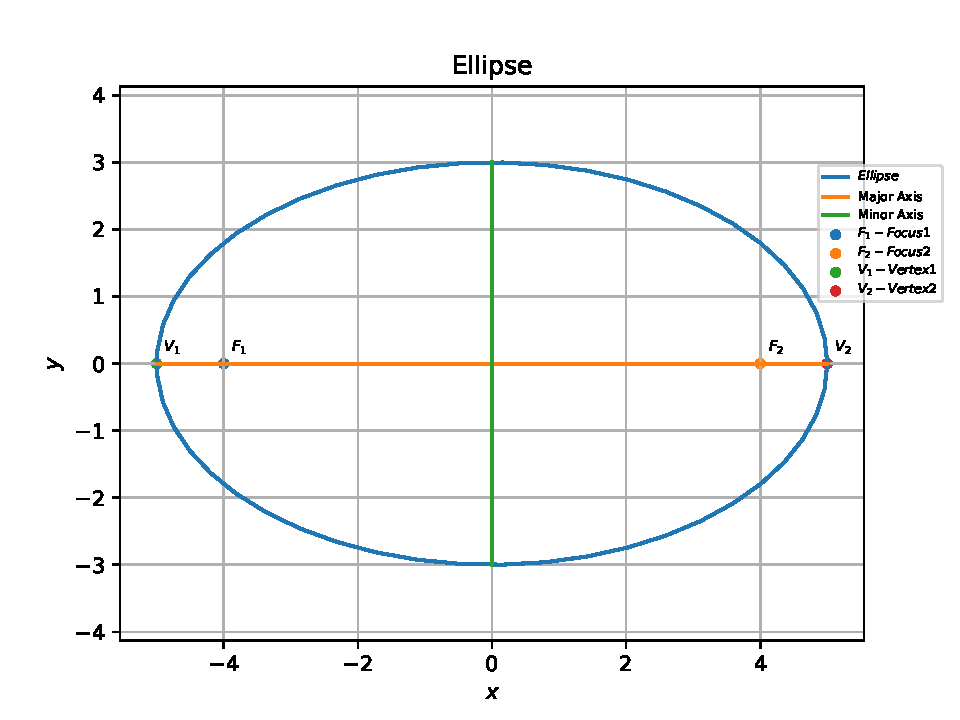
\includegraphics[width=\columnwidth]{chapters/11/11/5/7/figs/problem7.pdf}
	\end{center}
\caption{}
\label{fig:chapters/11/11/5/7/Fig1}
\end{figure}
